\documentclass{mcmthesis}
\mcmsetup{CTeX = false,   % 使用 CTeX 套装时，设置为 true
        tcn = 第12小组, problem = 工程问题,
        sheet = true, titleinsheet = true, keywordsinsheet = true,
        titlepage = false, abstract = true}
% \usepackage{newtxtext,newtxmath}
\usepackage{palatino}
\usepackage{lipsum}
\usepackage{algorithm}
\usepackage{algpseudocode}
\usepackage{tabularray}
\usepackage{color}
\usepackage{ctex}
\usepackage{caption}
\usepackage{graphicx}
\usepackage{float} 
\usepackage{subcaption}

% \usepackage{amsmath}
% \usepackage{hyperref}
\title{基于层次分析法和熵权TOPSIS法对中国、法国、美国的工程教育进行分析评价}

\begin{document}
\begin{abstract}
	
本文旨在运用\textbf{层次分析法}（AHP）与\textbf{熵权TOPSIS法}，对中国、法国及美国在工程教育领域的表现进行深入的剖析与评估。为全面反映各国\textbf{工程教育}的真实水平，我们精心选取了在该领域具有代表性的三所顶尖学府：中国的\textbf{清华大学}、美国的\textbf{麻省理工学院}以及法国的\textbf{巴黎综合理工学院}。通过教学质量、科研质量、创新成果和社会声誉这四个核心一级指标，以及它们所包含的16个二级指标。本文力求揭示三国工程教育的鲜明特色、显著优势及潜在不足，以期为中国工程教育的改革与发展提供有益的参考与启示。

\textbf{关键词：}层次分析法; 熵权TOPSIS法;工程教育;清华大学;麻省理工学院;巴黎综合理工学院
\begin{center}
	\textbf{Summary}
\end{center}

The purpose of this paper is to use the \textbf{analytic hierarchy process} (AHP) and \textbf{entropy weight TOPSIS method} to analyze and evaluate the performance of China, France and the United States in the field of \textbf{engineering education}. To fully reflect the true level of engineering education in each country, we have carefully selected three top universities that are representative of the field: \textbf{Tsinghua University} in China, \textbf{Massachusetts Institute of Technology} in the United States, and\textbf{ École Polytechnique} in France. Through the four core first-level indicators of teaching quality, scientific research quality, innovation achievements and social reputation, as well as the 16 second-level indicators contained in them, this paper aims to reveal the distinctive characteristics, significant advantages and potential shortcomings of engineering education in the three countries, in order to provide useful reference and enlightenment for the reform and development of engineering education in China.
\begin{keywords}
Analytic Hierarchy Process; Entropy Weight TOPSIS method; Engineering Education; Tsinghua University; Massachusetts Institute of Technology; École Polytechnique
\end{keywords}
\end{abstract}
\maketitle

\newpage

%%\section为一级标题，\subsection为二级标题 \subsubsection为三级标题
\section{引言}
随着全球化的深入发展，工程教育作为支撑国家科技进步和产业升级的重要基石，其地位愈发凸显。中国、法国和美国，作为世界工程教育的领军者，各自在工程教育领域都积淀了深厚的底蕴，形成了独具特色的教育模式。因此，对这三个国家的工程教育进行深入研究和比较，不仅有助于我们把握全球工程教育的发展趋势，更能为各国工程教育的改革与发展提供有益的参考。 \par
中国的工程教育近年来蓬勃发展，以清华大学为代表的一批顶尖学府，在工程教育领域取得了举世瞩目的成就。这些学府注重培养学生的创新能力和实践能力，通过校企合作、产学研一体化等模式，为学生提供了广阔的实践平台。同时，中国工程教育还积极培养学生的国际视野和跨文化交流能力，以适应全球化时代的挑战。 \par
法国的工程教育则以严谨、务实的风格著称。法国高校在工程教育中强调理论与实践的紧密结合，为学生提供了丰富的实验和实践机会。同时，法国工程教育还注重培养学生的跨学科思维和创新精神，以适应快速变化的市场需求。巴黎综合理工学院作为法国工程教育的典范，其先进的教育理念和教学方法为全球工程教育提供了宝贵的借鉴。 \par
而美国的工程教育则以其开放、创新的精神享誉全球。美国高校在工程教育中鼓励学生积极参与科研项目和实践活动，培养学生的创新能力和实践能力。同时，美国工程教育还注重培养学生的团队合作和沟通能力，以适应复杂多变的工程环境。麻省理工学院作为美国工程教育的领军者，其卓越的教育质量和创新成果为全球工程教育树立了新的标杆。\par
通过对中国、法国和美国三国工程教育的对比分析，我们可以发现，虽然各国在工程教育理念、教学方法等方面存在差异，但这些差异正是各国在工程教育领域不断探索和创新的结果。深入研究和分析这些差异，有助于我们更全面地了解全球工程教育的发展趋势和未来方向，为中国工程教育的改革与发展提供有益的启示和借鉴。\par

\section{问题介绍}
工程教育作为一个复杂且多维度的系统，涉及教学质量、研究质量、创新产出和社会声誉等多个方面。如何对这些方面进行科学、客观的评价，一直是工程教育领域亟待解决的问题。本研究致力于深入探讨中、法、美三国在工程教育领域所展现的独特特色与显著优势，同时，也深入剖析中国在工程教育方面尚存的不足之处与劣势，以期通过借鉴外国的先进经验，推动中国工程教育的持续发展与完善。\par

\section{理想化假设}
 为了简化给定的问题并使其更适合模拟现实条件，我们提出了以下基本假设，每个假设都有适当的理由。
\begin{itemize}
	\item 代表性假设：假设中国、法国和美国在各自工程教育领域顶尖的大学可以代表三国的工程教育水平。
	\item 稳定性假设：假设在短时间内，这三所大学的工程教育水平保持相对稳定，没有发生显著变化，这样比较结果才具有参考价值。
	\item 评价标准假设：假设各大学在工程教育方面的评价标准和方法在一定程度上是一致的，这样可以确保比较结果的公正性和准确性。
\end{itemize}

\section{符号说明}
\begin{table}[h]
	\centering
	\caption*{ 本论文中所有符号说明}
	\begin{tblr}{
			column{9} = {c},
			column{13} = {c},
			hline{1-2,7} = {-}{},
		}
		&  &  &  &  &  &  &  & 符号 &  &  &  & 说明 &  &  &  &  &  &  &  &  \\
		&  &  &  &  &  &  &  & $e$      &  &  &  & 信息熵       &  &  &  &  &  &  &  &  \\
		&  &  &  &  &  &  &  & $d$ &  &  &  & 差异度       &  &  &  &  &  &  &  &  \\
		&  &  &  &  &  &  &  & $W$      &  &  &  & 权重        &  &  &  &  &  &  &  & \\ 
		&  &  &  &  &  &  &  & $i$      &  &  &  & 国家索引        &  &  &  &  &  &  &  & \\ 
		&  &  &  &  &  &  &  & $j$      &  &  &  & 指标索引       &  &  &  &  &  &  &  &  



	\end{tblr}
\end{table}
\section{思路介绍}
\subsection{评价指标体系构建}
经过细致的文献梳理与资料分析，我们成功构建了一个全面而系统的工程教育评价指标体系。这一体系不仅包含了四个核心一级指标，还细化了十二个二级指标，以全面而深入地剖析工程教育的各个层面。该体系的构建过程如图一所示，我们确保了其科学性与准确性，为后续深入分析和比较不同国家的工程教育特色与优劣奠定了坚实的基础。本研究所采用的一级指标以及相关配重均引自权威文献《多元分类视角的高等工程教育评价指标体系构建及其应用——以97所“双一流”建设高校为样本》\cite{1}。
\begin{figure}[h]
	\small
	\centering
	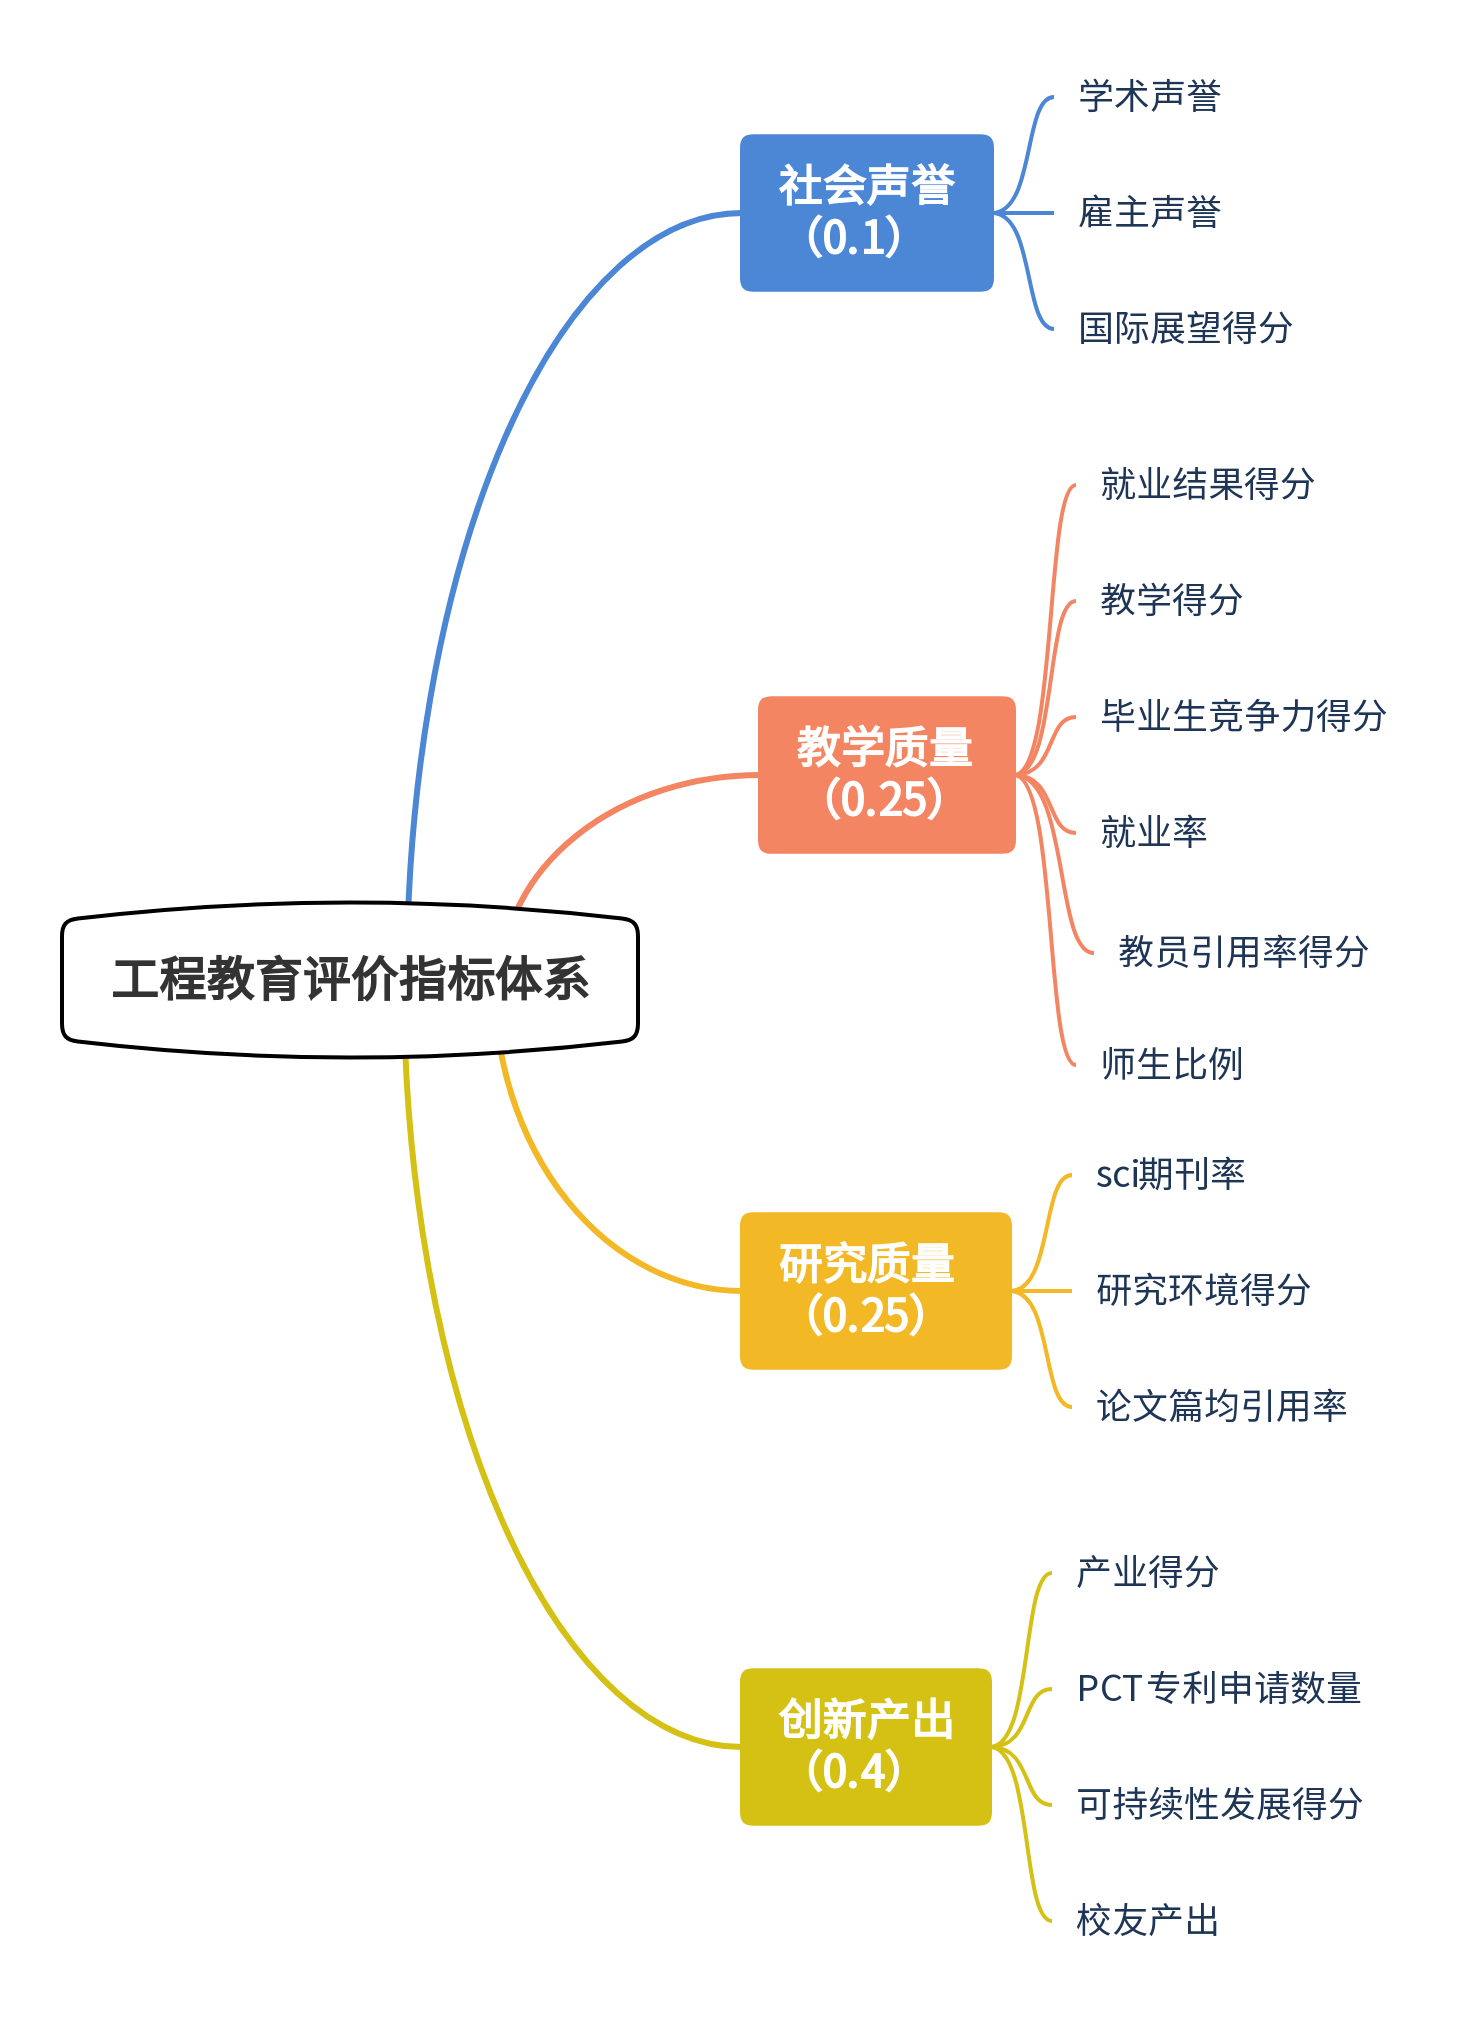
\includegraphics[width=12cm]{pingjiazhibiao.png}
	\caption{工程教育评价指标体系}
\end{figure}
\subsection{方法选择}
在研究方法的选择上，我们综合考虑了多种因素，最终确定了熵权法TOPSIS和层次分析法作为本研究的分析模型。熵权法TOPSIS能够基于数据的客观变异程度确定各指标的权重，避免了主观因素的干扰，确保了评价结果的客观性。同时，TOPSIS法作为一种多属性决策分析方法，能够全面考虑各个指标，并有效计算出各方案之间的相对优劣，为我们提供了清晰的比较依据。而层次分析法则结合了定性与定量的分析方法，能够充分利用专家的经验和判断，将复杂问题分解为多个层次和因素，形成递阶层次结构，便于我们系统地分析和评价三国工程教育的特色和优劣。这种方法不仅提高了决策的准确性和科学性，还使得我们的分析更加深入和系统。在本研究中，对于二级指标的权重以及其所属一级指标的得分计算，我们将采用熵权法TOPSIS，避免主观干扰。然后将一级指标作为准则层，三个国家的工程教育作为方案层，通过层次分析法，得到决策目标。
\section{方法实现}
\subsection{数据收集}
\subsubsection{确定数据收集对象}
\begin{itemize}
	\item 在筛选各国工程教育领域的顶尖综合类大学时，我们发现中国的清华大学凭借其卓越的工科实力脱颖而出。清华大学的A类工科占据全校A类学科的半壁江山，高达54.1\%，同时其工科类学科中，超过八成被评为A类，这一比例高达83.3\%。清华的工科专业特色鲜明，实力强劲，相较于北京大学，其工科优势更为显著，北大的A类工科仅占全校A类学科的14.3\%\cite{2}。因此，我们毫不犹豫地选择了清华大学作为中国工程教育的代表。
	\item 在美国，麻省理工学院（MIT）在工程教育领域的卓越地位更是无可争议。该校在工程技术类专业上已经连续18年蝉联世界第一，这一骄人的成绩充分展现了麻省理工学院在工程教育领域的卓越成就和全球影响力，使其成为了美国工程教育的典范。
	\item 至于法国，巴黎综合理工学院无疑是该国工程教育的领军者。在《学生报》发布的2024年工程师学院排名中，该校稳居榜首，充分证明了其强大的教育实力。巴黎综合理工学院不仅注重培养学生的实践能力和创新精神，还致力于为法国乃至全球的工程界输送优秀的专业人才，其影响力与贡献不容忽视。
\end{itemize}
\par
因此，我们分别选择，清华大学，麻省理工学院，巴黎综合理工学院的工程教育水平来代表这三个国家。
\subsubsection{原始数据展示}
\begin{figure}[h]
	\small
	\centering
	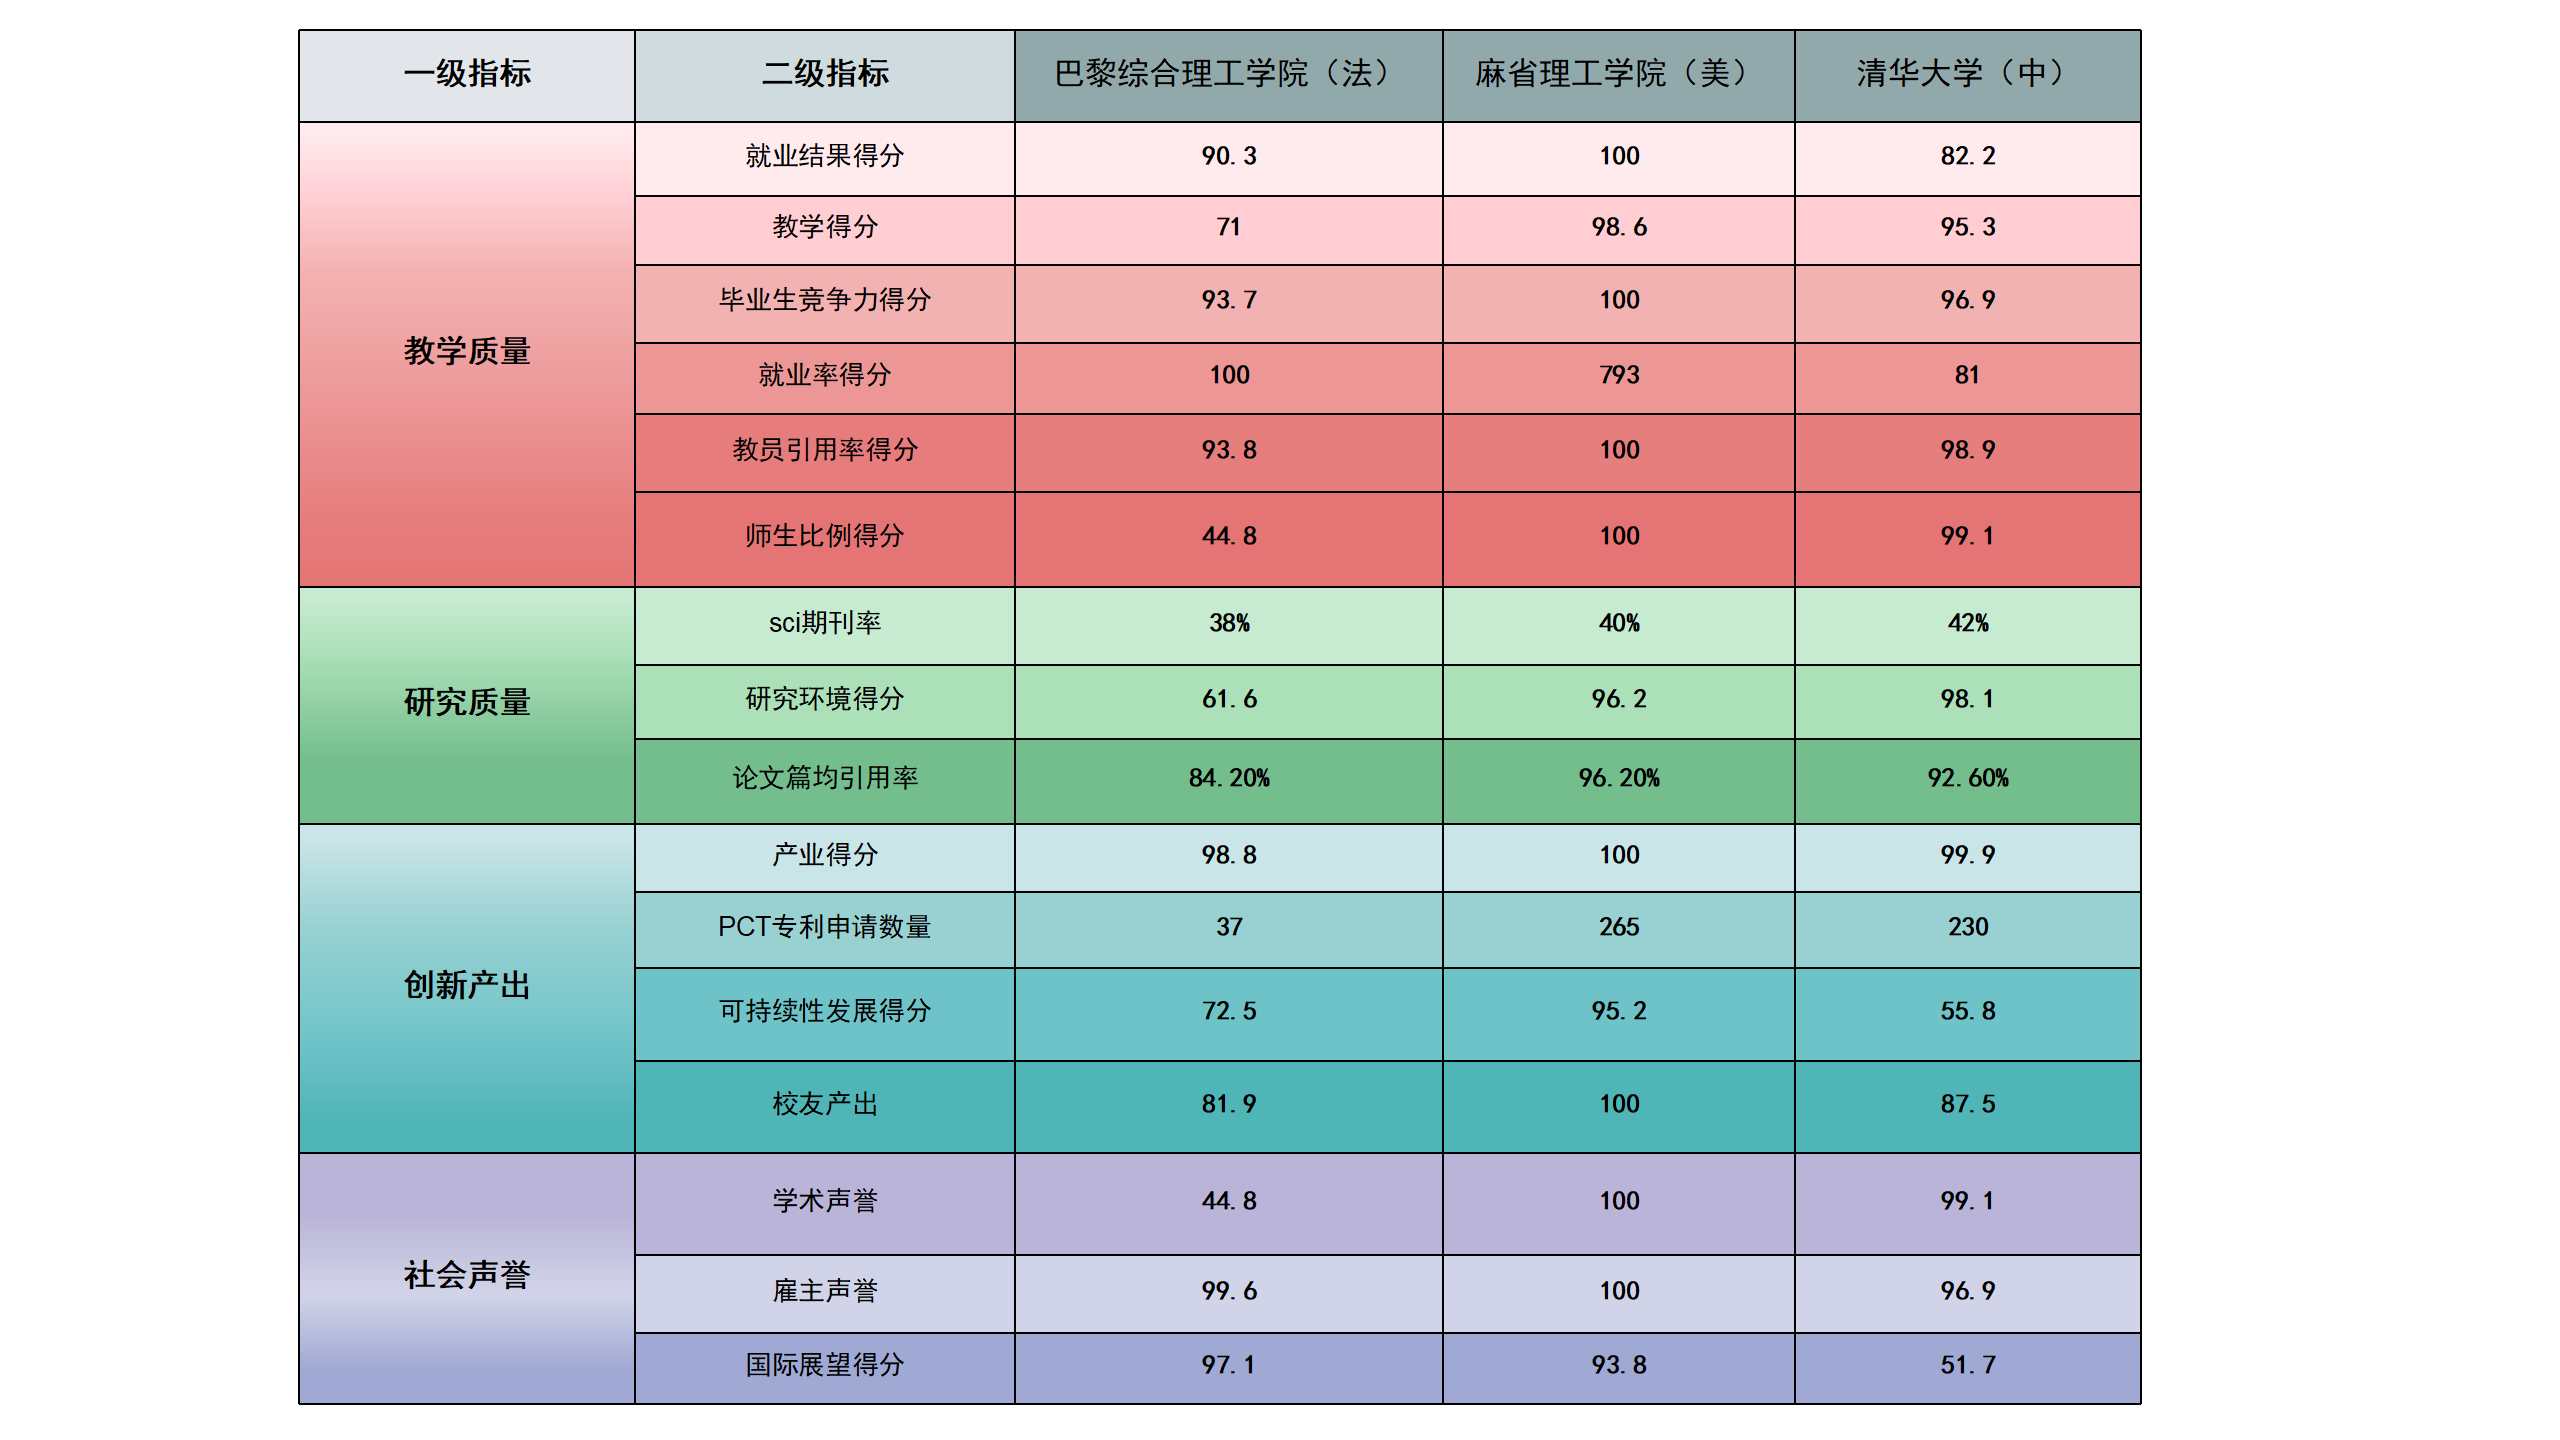
\includegraphics[width=16cm]{yuanshishuju.png}
	\caption{原始数据图}
\end{figure}
\par
数据来源：泰晤士大学排名\cite{3}；2023-2024QS世界大学排名(QS World University Rankings)\cite{4}；incopat数据库等。		
\subsection{数据处理}
\subsubsection{熵权TOPSIS}
首先，为了去除量纲以及数据尺度范围的影响，我们对每一横行的指标进行数据标准化处理。
$$
z_{i j}=x_{i j} / \sqrt{\sum_{i=1}^n x_{i j}^2}
$$
\par
然后，为了得到二级指标对于所属一级指标分数贡献率及权重的大小，我们分别对四个一级指标所包含的二级指标进行熵值法处理。得到他们对于所属一级指标的贡献率。

$$
e_j=-\frac{1}{\ln n} \sum_{i=1}^n p_{i j} \ln \left(p_{i j}\right)(j=1,2, \cdots, m)
$$
\par
对于第j个指标而言，其信息熵$e_j$可以使用上式得到。其中,i是三个大学的索引，此处n为大学数量3。之后，通过$d_j=1-e_j$得到该指标的差异度指数。再由下式得到对应权重。$$
W_j=d_j / \sum_{j=1}^m d_j(j=1,2, \cdots, m)
$$
\par
其中m为一级指标所属二级指标的个数。对于教学质量来说m=6,研究质量m=3，以此类推，得到了图3。

\begin{figure}[h]
	\small
	\centering
	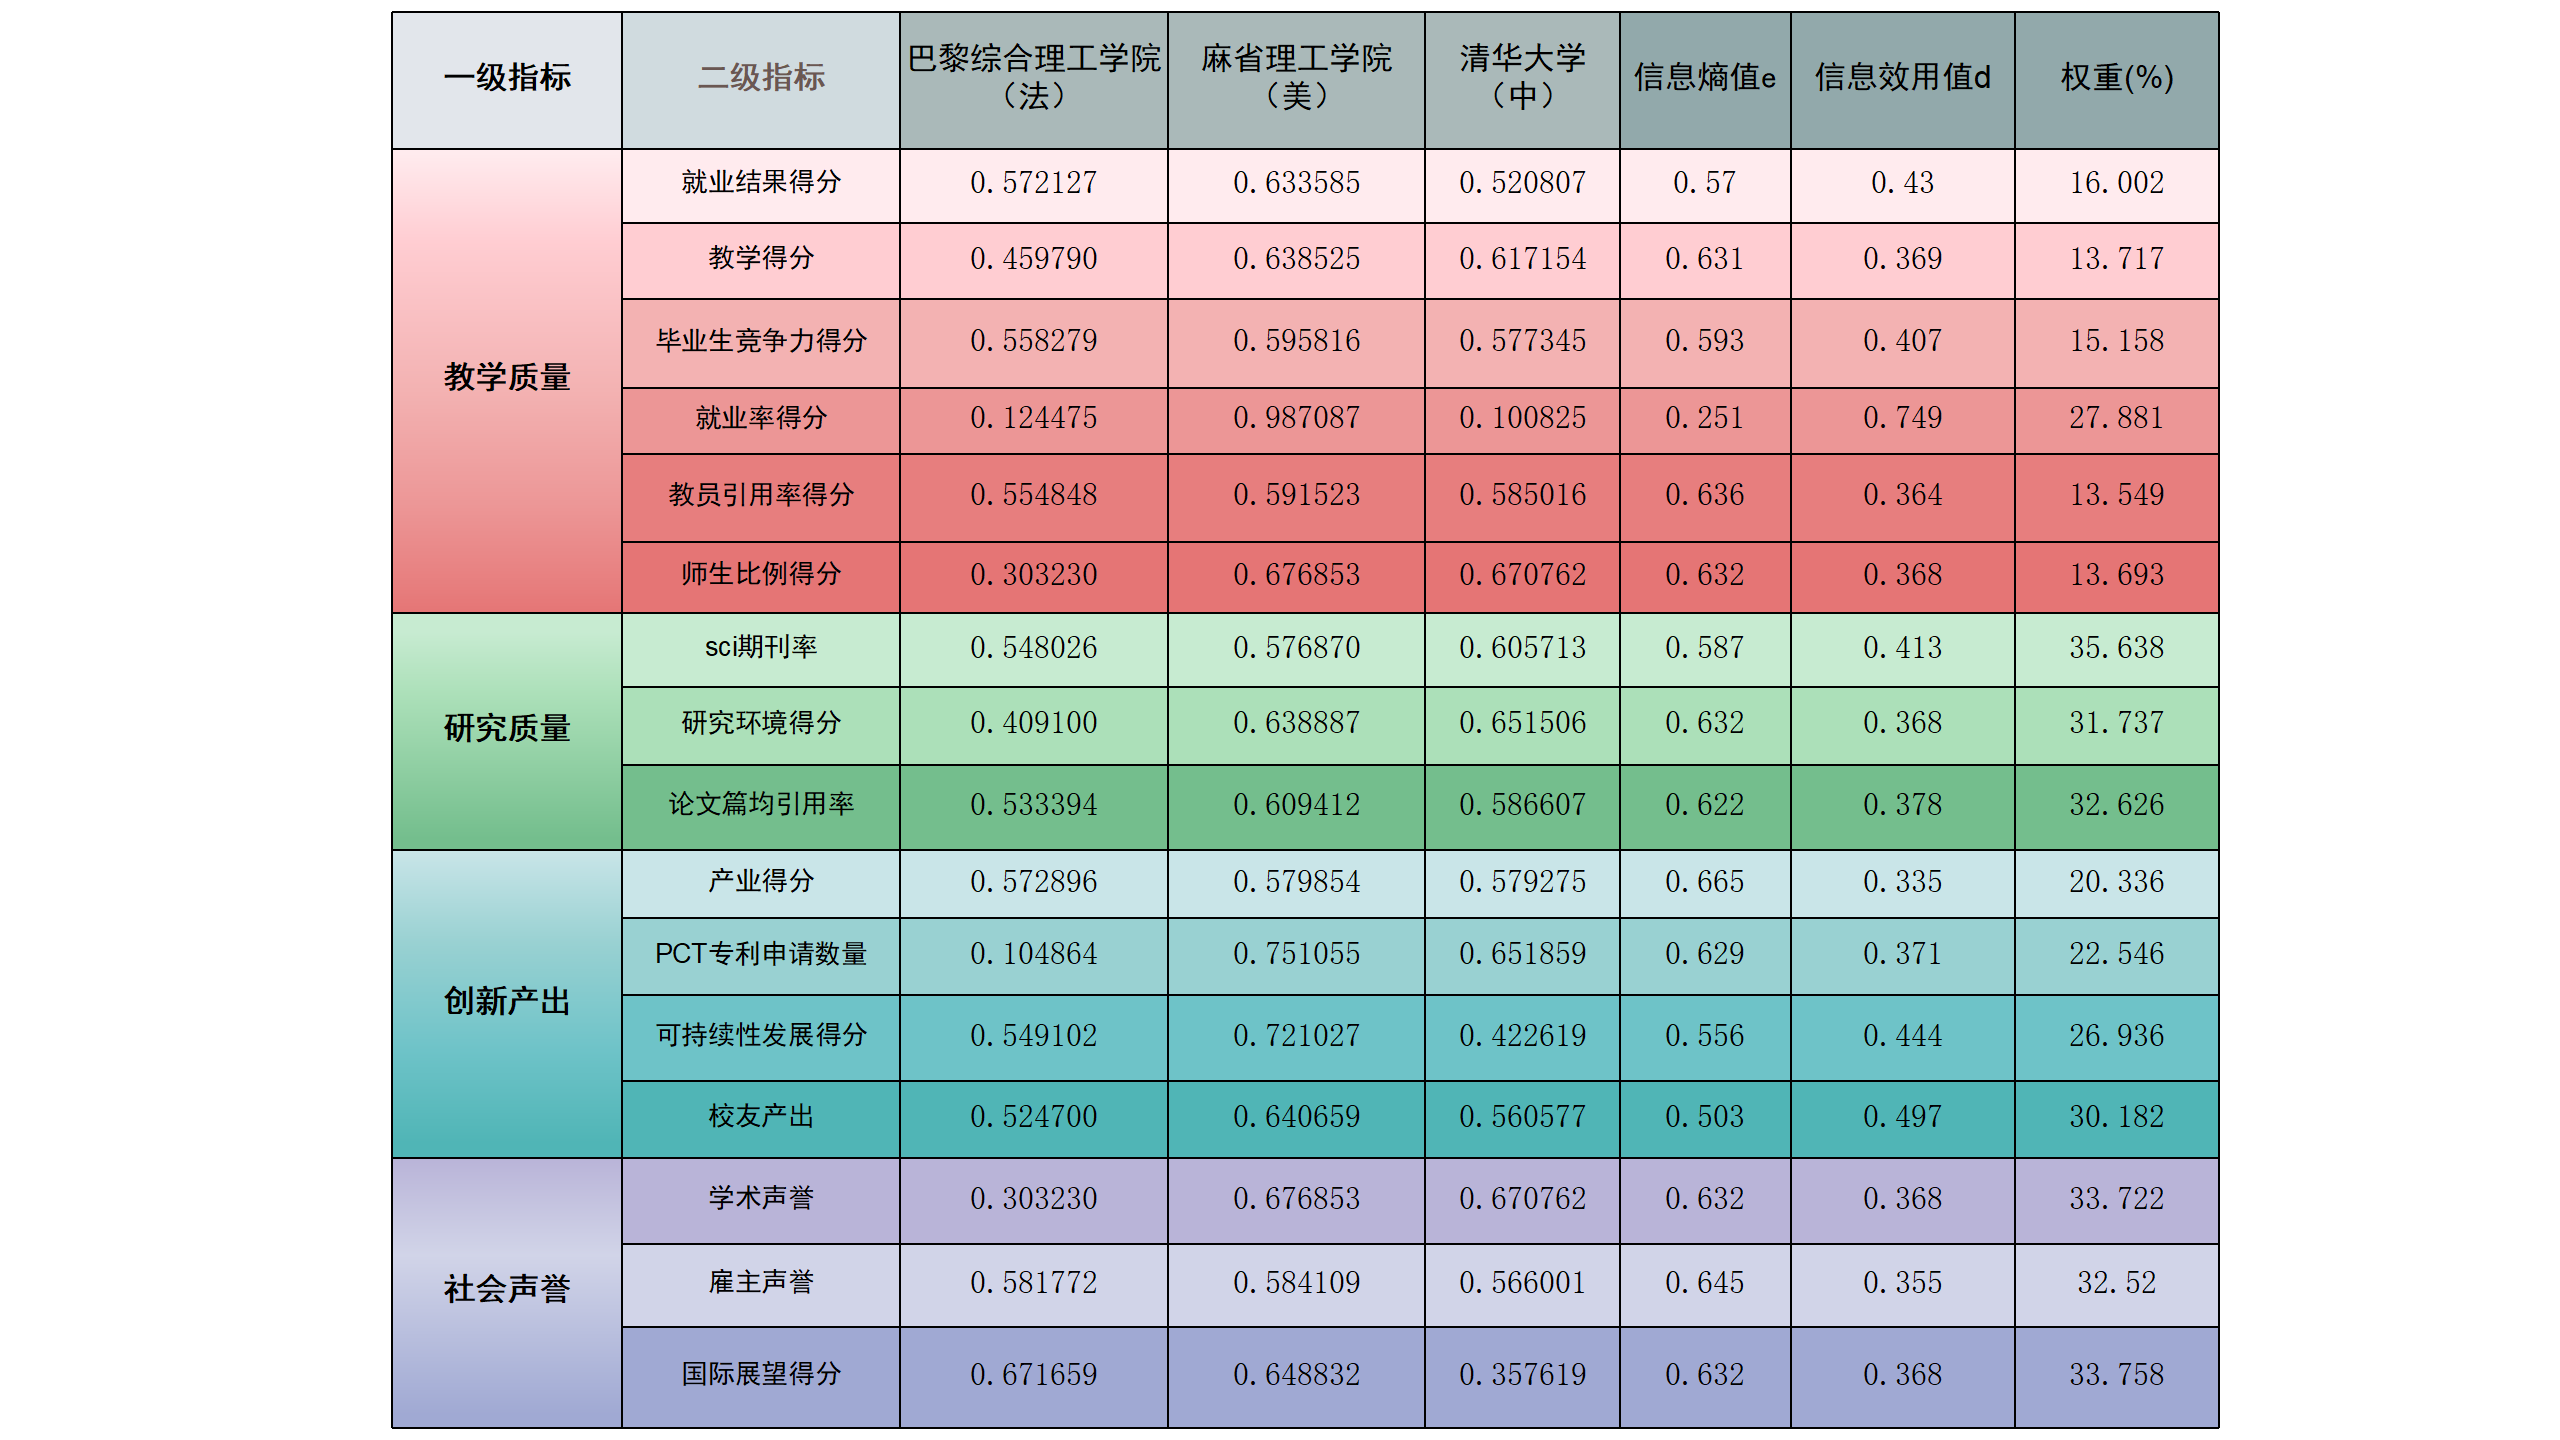
\includegraphics[width=15cm]{jiagongshuju.png}
	\caption{处理后的数据图}
\end{figure}
\par 
各学校，在其每个一级指标下所属的二级指标分数加权求和，即可得到，各学校分别在四个一级指标上的分数。
\subsubsection{层次分析法}
\par
在得到一级指标的分数后，便成一个简单的决策问题，如图4所示。
\begin{figure}[h]
	\small
	\centering
	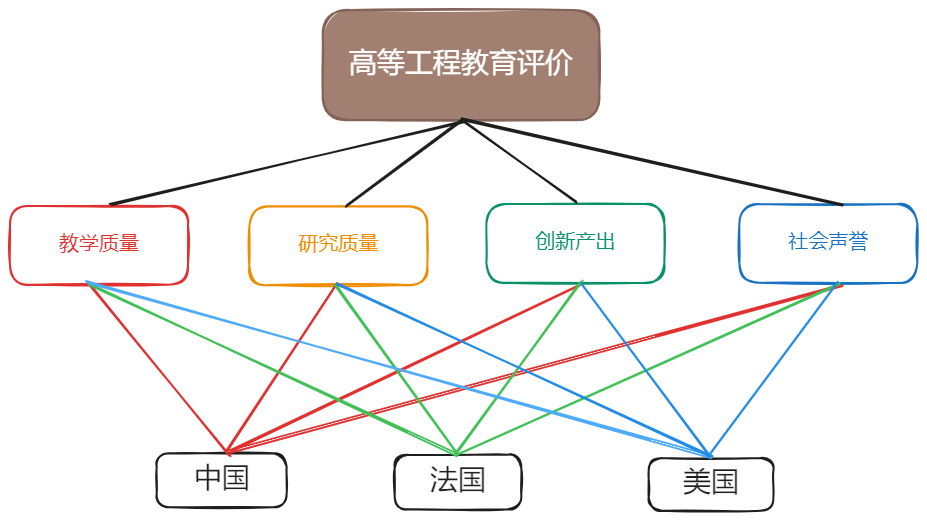
\includegraphics[width=14cm]{cengcifenxi.png}
	\caption{层次分析决策图}
\end{figure}
\par
准则层即为4个一级指标，这四个指标及其权重全部引自《多元分类视角的高等工程教育评价指标体系构建及其应用——以97所“双一流”建设高校为样本》\cite{1}一文。在此文中，运用层次分析法，通过在多所高校调查，得到该权重，如图5所示。
\begin{figure}[h]
	\small
	\centering
	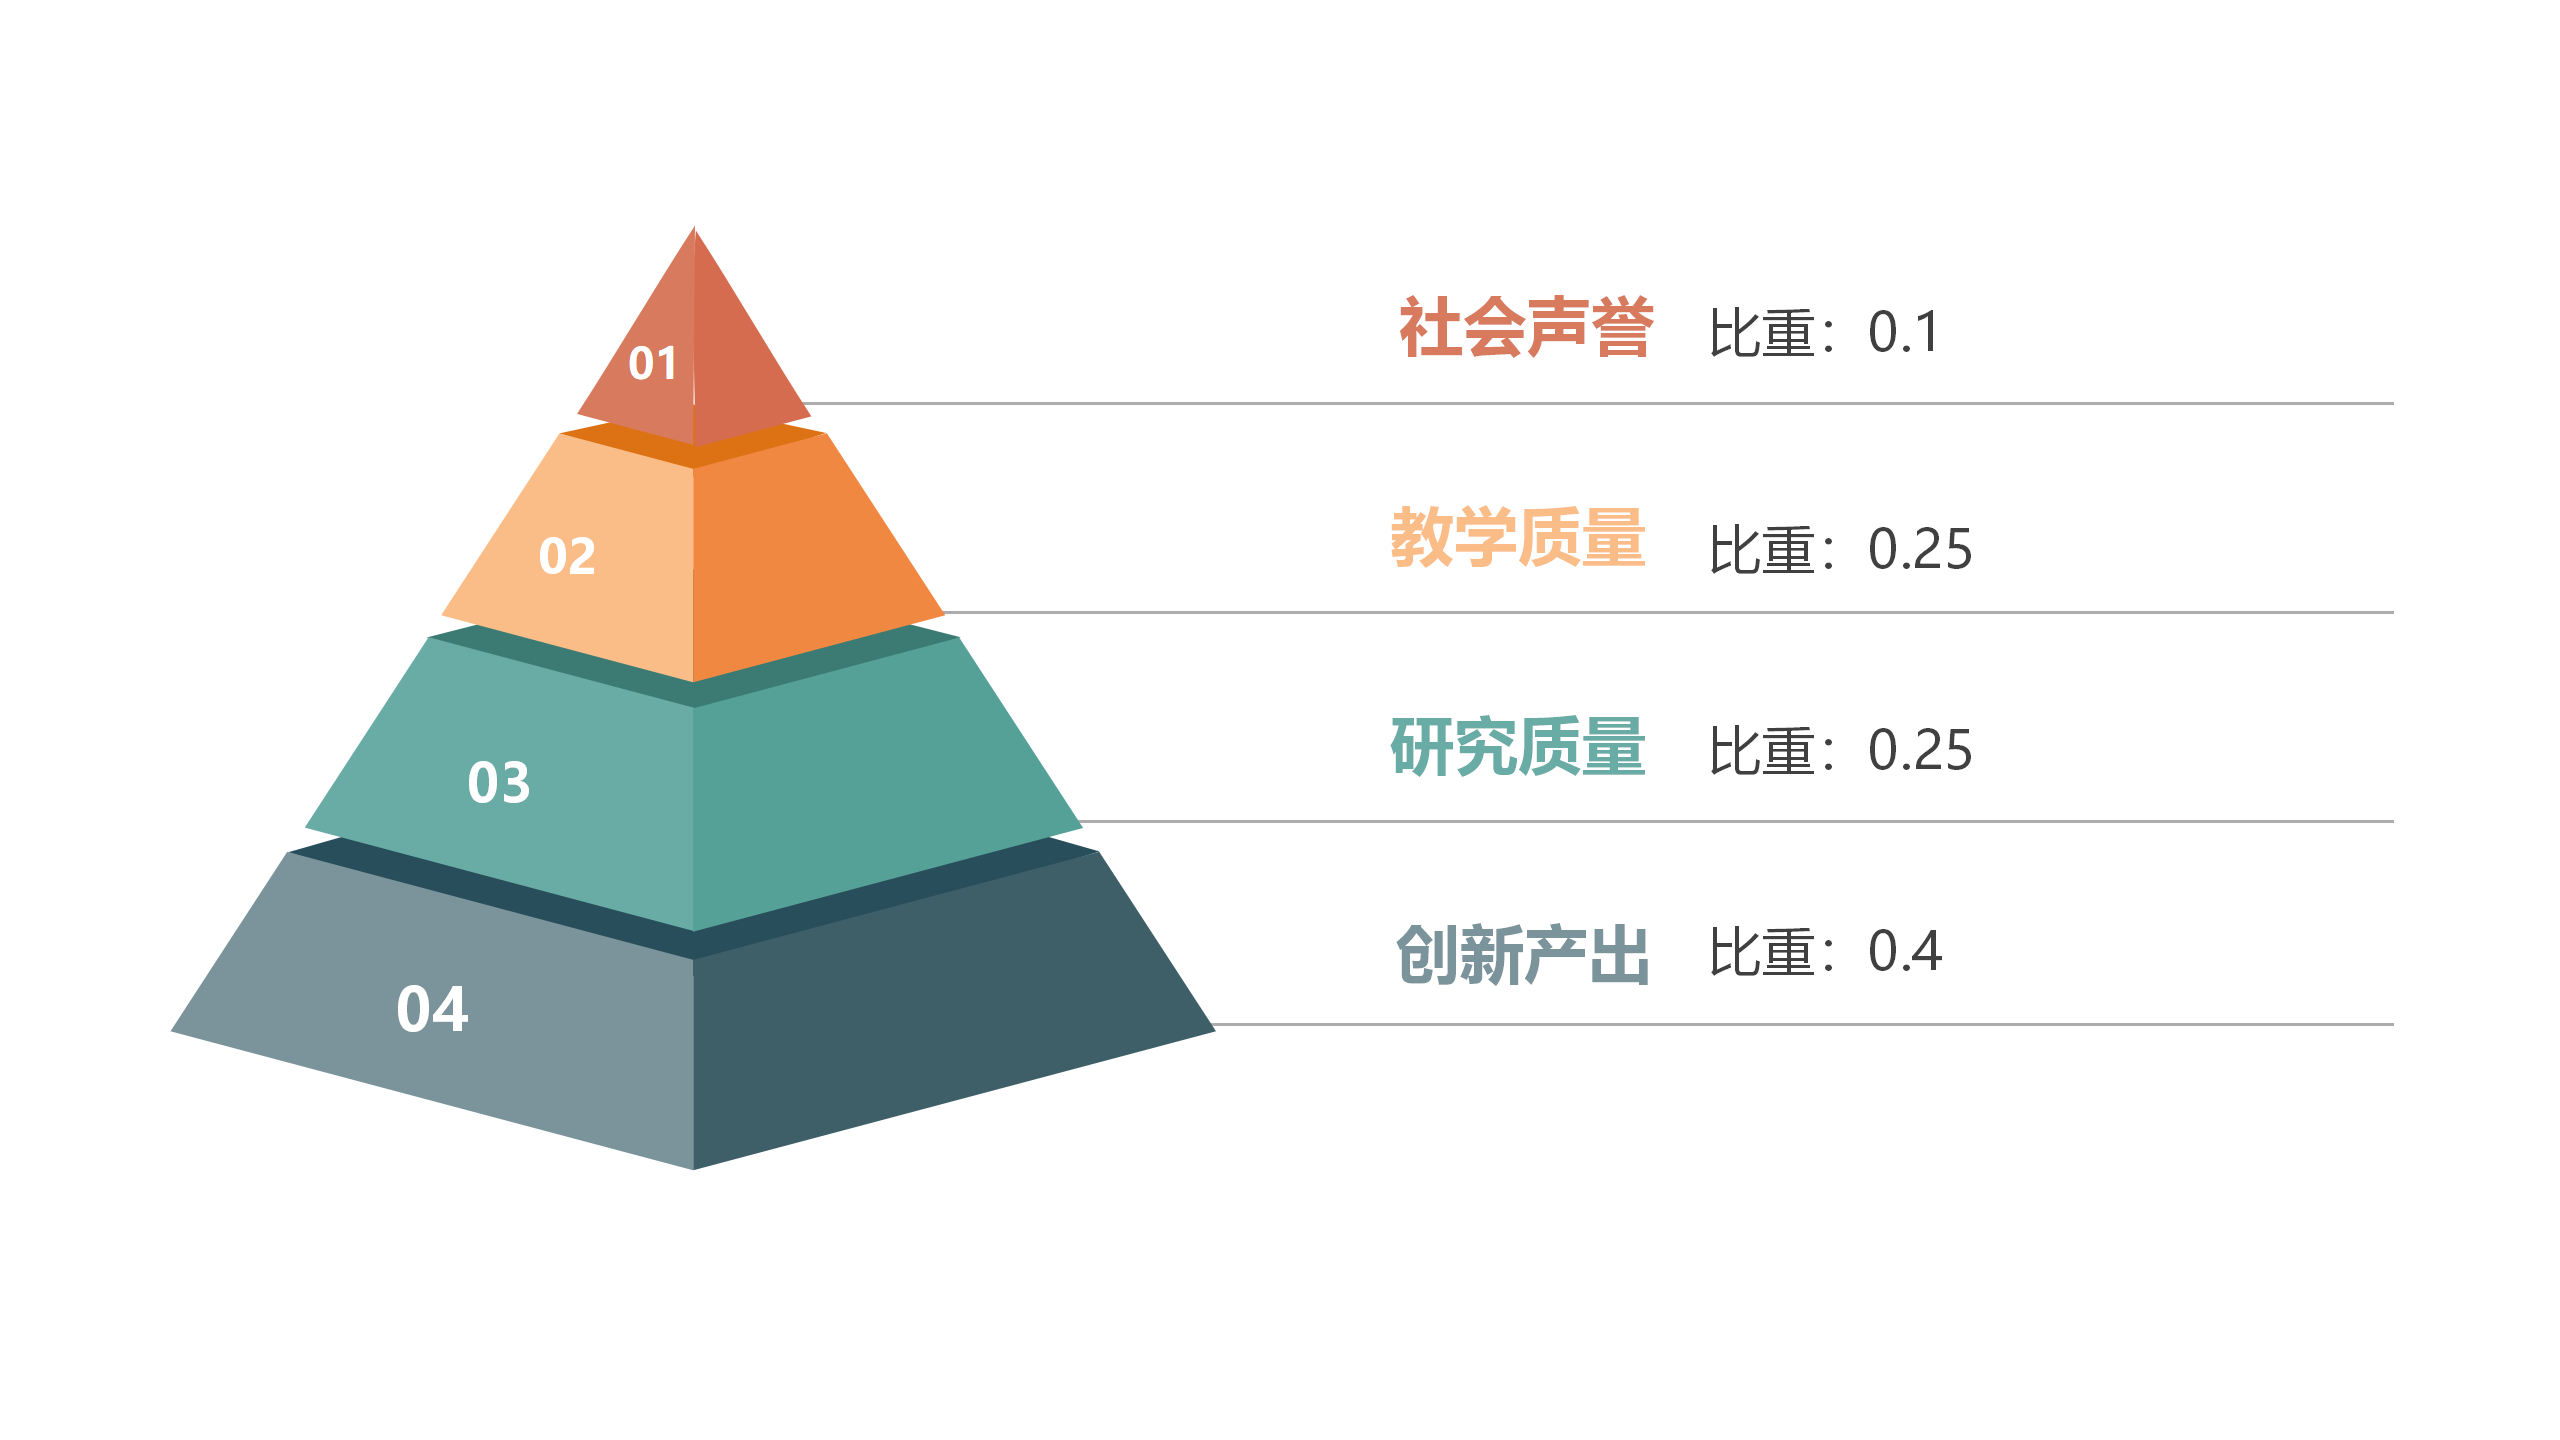
\includegraphics[width=13cm]{yijiquanzhong.png}
	\caption{权重金字塔}
\end{figure}

三所大学分别对四个一级指标加权求和，得到最终每所大学在工程教育领域的得分。分别表示三个国家的工程教育水平，如图6所示。
\begin{figure}[h]
	\small
	\centering
	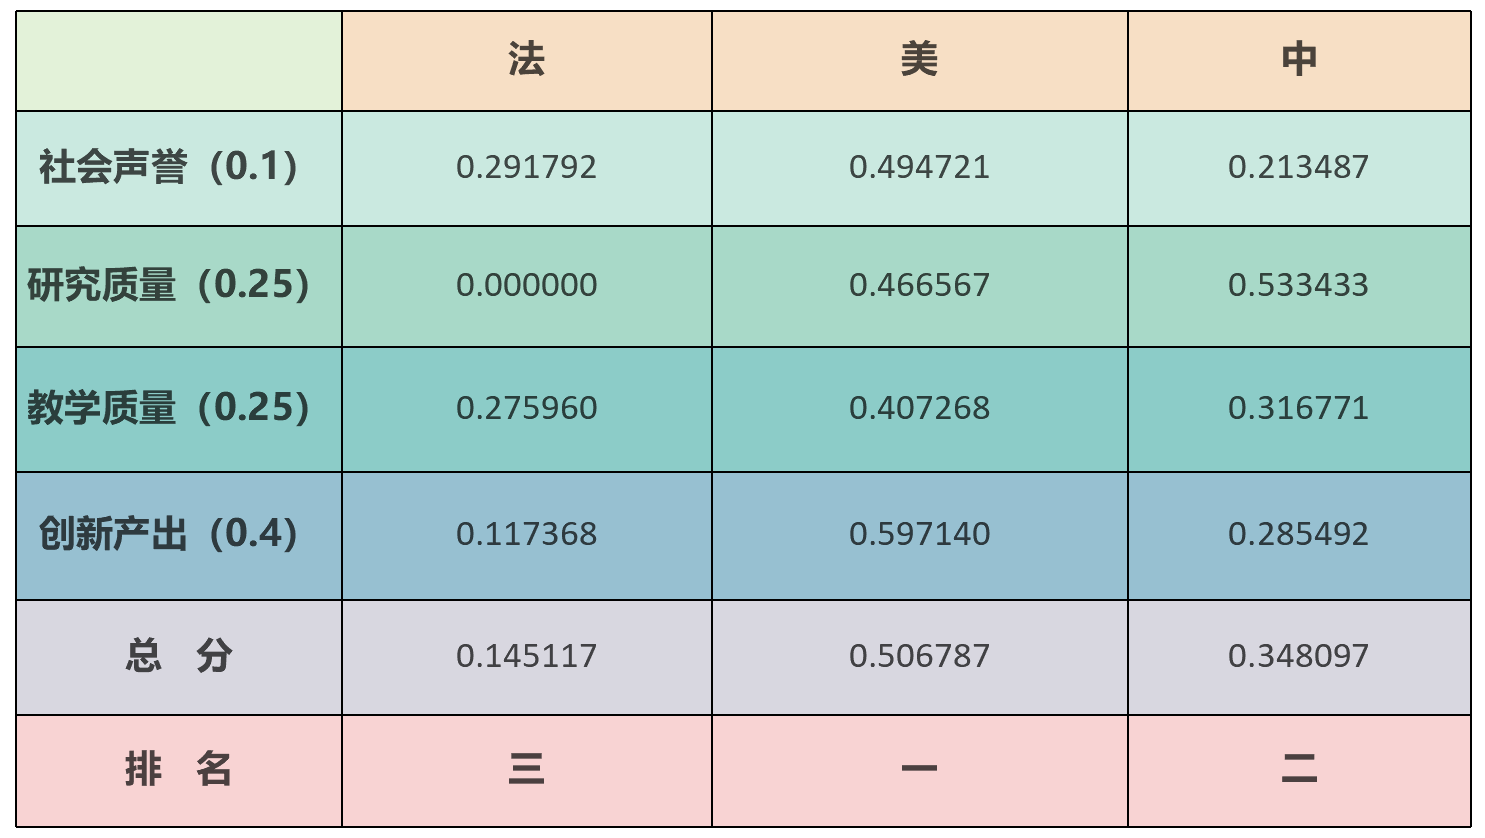
\includegraphics[width=15cm]{zuizhongdefen.png}
	\caption{中法美三国工程教育最终得分}
\end{figure}
\section{结论}

观察图6，通过总体评价与各维度的评价可以得到以下结论。
\begin{itemize}
	\item 总体评价：美国工程教育综合得分大于中国综合得分，大于法国综合得分。即中国与法国的工程教育水平总体相对于美国仍有差距，需要努力。
	\item 单个维度：中国工程教育水平研究质量方面领先，而在其他三个维度仍然落后于美国，需要针对这些方面加强提升。
	\item 结论：美国工程教育在综合评价中表现最优，其工程教育在多个方面均达到了较高的水平。中国和法国的工程教育也表现出色，有自己的优势，但在某些方面仍有提升空间。未来，我们可以进一步拓展研究范围，纵横纳入更多国家及其顶尖大学，以更全面地了解全球工程教育的发展趋势和特点
\end{itemize}
\section{方法缺陷分析}

在方法上，本研究虽然采用了熵权法TOPSIS和层次分析法对工程教育进行了深入分析，但仍存在一些局限性。首先，以三所顶尖高校代表整个国家的工程教育水平可能不够全面。其次，数据来源和质量可能存在一定的差异和偏差。此外，权重确定过程中存在一定的主观性和对特殊情况的不敏感性。因此，在后续研究中应进一步拓展数据源，完善指标体系，以提高研究的准确性和可靠性。


\begin{thebibliography}{99}
\bibitem{1}张炜,邓勇新,辛越优,等. 多元分类视角的高等工程教育评价指标体系构建及其应用——以97所“双一流”建设高校为样本 [J]. 中国高教研究, 2021, (02): 10-15. DOI:10.16298/j.cnki.1004-3667.2021.02.03.
\bibitem{2} 优志愿. 大学白皮书：清华和北大到底哪个好？院校综合实力对比分析. 知乎.https://zhuanlan.zhihu.com/p/87935232。
\bibitem{3}泰晤士高等教育(Times Higher Education).2023年世界大学排名.https://www.timeshighereducation.com/cn/world-university-rankings。
\bibitem{4}QS世界大学排名. 2023年世界大学排名. https://www.qschina.cn/university-rankings/world-university-rankings/2023。

\end{thebibliography}

\end{document}

